%%%%%%%%%%%%%%%%%%%%%%%%%%%%%%%%%%%%%%%%%%%%%%%%%%%%%%%%%%%%
%%%%%%%%%%%%%%%%%%%%%%%%%%%%%%%%%%%%%%%%%%%%%%%%%%%%%%%%%%%%
\section{Introduction}
%%%%%%%%%%%%%%%%%%%%%%%%%%%%%%%%%%%%%%%%%%%%%%%%%%%%%%%%%%%%
%%%%%%%%%%%%%%%%%%%%%%%%%%%%%%%%%%%%%%%%%%%%%%%%%%%%%%%%%%%%

\subsection{Contexte}
Cette étude s'inscrit dans le cadre du projet Fouille de données. L'objectif est de mettre en oeuvre notre capacité à adopter une démarche efficace et interessante pour analyser un jeu de données concernant un certain nombre de pays.

Nous avons, pour cela, à notre disposition trois jeux de données sous forme de fichiers CSV\footnote{\verb!countries2007\_all.csv!, \verb!countries2007\_noMissing1.csv!, \verb!countries2007\_noMissing2.csv!}. Ces trois fichiers contiennent de nombreuses informations sur un certain nombre de pays. Nous avons restreint notre étude au fichier \verb!countries2007_noMissing1.csv! qui ne contient que 88 entrées pour 32 attributs, mais présente l'avantage de proposer des valeurs pour chaque couple \og pays -- attribut \fg.

En ce qui concerne les outils utilisés, un logiciel de fouille de données présenté en séance nous permet d'effectuer differentes explorations : il s'agit de \textsc{knime}\footnote{\url{http://www.knime.org/}}. 

\subsection{Problématique}

Les mouvements révolutionaires de libération que connait le monde arabe nous ont poussé à étudier de plus près l'impact des libertés civiles sur les situations sociale, économique et militaire de certains pays, ou du moins la corrélation entre ces deux groupes de caractéristiques.
Après l'introduction d'un nouvel attribut au jeu de donnés que nous possédons, nous nous poserons la question de savoir s'il y a un lien entre ce nouvel indicateur (indice de liberté) et les données démographique, militaire, économique, sociale, ou autres, d'un pays.
On s'intéressera par la suite à retrouver cet indice de liberté à partir d'un ensemble de données définis durant l'étude précédente. En d'autres termes, nous essaierons de corroborer les différents résultats de la première partie, s'il y a lieu, en retrouvant l'indice de liberté de certains états et en le comparant aux données de notre source d'informations initiale.



%%%%%%%%%%%%%%%%%%%%%%%%%%%%%%%%%%%%%%%%%%%%%%%%%%%%%%%%%%%%
%%%%%%%%%%%%%%%%%%%%%%%%%%%%%%%%%%%%%%%%%%%%%%%%%%%%%%%%%%%%
\section{Détermination du champ d'étude}
%%%%%%%%%%%%%%%%%%%%%%%%%%%%%%%%%%%%%%%%%%%%%%%%%%%%%%%%%%%%
%%%%%%%%%%%%%%%%%%%%%%%%%%%%%%%%%%%%%%%%%%%%%%%%%%%%%%%%%%%%
\subsection{Identification des attributs pertinents}

Cette partie tentera de justifier les choix d'attributs pour leur rapport \emph{possible} avec la liberté civile des peuples.
Dans un premier temps, nous commencerons par constituer des groupes d'attributs sous forme de catégories (social, santé, armée, démographie, économie) en justifiant ce choix d'attributs à l'aide de leurs eventuels liens avec la liberté civile des peuples.
Après quoi, nous passerons à l'étude des corrélations des differents attributs d'un même groupe pour finalement aboutir au choix définitif.

\subsubsection{Social}
\begin{description}
\item [Adolescent fertility rate] 
Il est possible de supposer --- à la limite --- qu'un état totalitaire aura des particularités du point de vue de la fécondité des adolescents. En effet, on peut imaginer que le taux d'accès aux études supérieures plus bas influence 
\item [Worker's remittances and compensation of employees]
Reflet direct du niveau de vie des habitants, cet attribut serait dépendant de l'indice de liberté et s'illustrerait par des salaires et des primes très bas au sein d'une dictature militaire.
\item [Internet users]
Les aspects de censure liés aux dictatures se traduiraient par un usage très limité d'internet. Aussi le nombre d'internautes 
au sein d'une dictature se réduisant aux membres du régime, on s'attend à trouver une relation proportionnelle entre l'indice de liberté et le nombre d'internautes.
\item [Mobile cellular suscriptions]
Le fort contrôle des moyens de communication de la part d'un régime totalitaire pourrait induire une utilisation de la télphonie mobile très limitée.
\end{description}

\graph{correlation_social}{Corrélation linéaire des différents attributs choisis dans la catégorie \emph{Social}}
Les attributs ayant trait aux nouvelles technologies de l'information sont linéairement corrélés, pour des raisons évidentes. De manière plus surprenante, la fécondité des adolescents semble se rapprocher d'une fonction linéaire décroissante du taux d'accès à Internet\ldots
Sans nous livrer à des conclusions trop hâtives, nous ne considérerons cependant que le taux d'accès Internet en tant qu'attribut représentant les trois.

\subsubsection{Santé}
\begin{description}
\item [Immunization, measles]
Cet attribut est étroitement lié aux impacts de la liberté sur les aspects économiques d'un pays. Un pays totalitaire
accorderait peu d'importance aux achats (imports ?) de vaccins contrairement aux investissements de l'armement militaire.
\item [Life expectancy at birth, total]
On pourrait croire que les libertés d'un pays influencent l'esperance de vie de sa population. Cette hypothèse serait une conséquence
des autres attributs qui lieraient liberté aux aspects économiques et sociaux d'un pays. En d'autres termes, moins un pays est libre plus sa situation sociale et sanitaire se dégrade, plus l'espérance de vie décroit.
\item [Mortality rate, under-5]
De même que pour l'espérance de vie, on peut supposer que le taux de mortalité des moins de 5 ans est une fonction croissante des libertés civiles d'un peuple.
\item [Prevalence of HIV, total]
Il est envisageable que le manque de liberté influence l'accès aux soins, par exemple en supposant qu'un pays sous pression politique soit peu développé.
\end{description}

\graph{correlation_sante}{Corrélation linéaire des différents attributs choisis dans la catégorie \emph{Santé}}
Comme tous les attributs sont corrélés entre eux (on peut trouver au maximum deux attributs ayant un coefficient de corrélation linéaire relativement faible), il est difficile de continuer l'étude sur ce seul groupe d'attributs. Nous verrons par la suite comment remédier à ce problème.

\subsubsection{Armée}
\begin{description}
\item [Adolescent fertility rate]
Cf plus haut.
\item [Military expenditure]
On prévoit de trouver un lien très fort entre les dépenses militaires et les libertés civiles d'un pays. Un pays totalitaire pourrait avoir de très importantes dépenses militaires et inversement.
\item [Fertility rate, total]
On s'attend à trouver un lien entre le taux de fécondité et la liberté. Un indice de liberté bas se traduirait peut-être par un taux de fécondité bas également et inversement.
\item [Life expectancy at birth, total]
Cf plus haut.
\item [Surface area]
Un grand pays en termes de surface pourrait être difficilement contrôlable par une dictature militaire. Il posséderait donc selon toute probabilité une liberté civile plus importante qu'un pays plus petit en surface.
\end{description}

\graph{correlation_armee}{Corrélation linéaire des différents attributs choisis dans la catégorie \emph{Armée}}
Sans surprise, le taux de fécondité des adolescentes est fortement lié à celui des femmes en général. De même, l'espérance de vie est fortement liée à ces taux de fécondité. On ne retiendra donc que l'espérance de vie.

\subsubsection{Démographie} 
\begin{description}
\item [Fertility rate]
Cf. plus haut.
\item [Adolescent fertility]
Cf. plus haut.
\item [Population, total]
On part de la même hypothèse que celle concernant la surface : plus la population est importante plus elle peut être incontrôlable, donc libre (en excluant des pays singuliers tels que la Chine).
\item [Population growth]
Tout comme le taux de mortalité, la croissance serait inversement proportionnelle à l'indice de liberté d'un pays.
\item [Life expectancy at birth, total]
Cf. plus haut.
\item [Surface area]
Cf. plus haut.
\end{description}

\graph{correlation_demographie}{Corrélation linéaire des différents attributs choisis dans la catégorie \emph{Démographie}}
Comme dans le domaine de la santé, les attributs sont corrélés dans des proportions déraisonnables. Ce problème est traité plus bas.

\subsubsection{Economie}
\begin{description}
\item [Agriculture, value added]
Parmi les impacts économiques d'une absence de liberté, on pourrait trouver une très forte participation de l'agriculture dans l'économie d'une dictature militaire.
\item [Exports of goods and services]
On s'attend à trouver une relation inversemment proportionnelle entre la capacité d'une dictature à exporter des services et des biens et l'indice de liberté de celle-ci.
\item [Foreign direct investment, net inflows]
Idem que pour les exportations. 
\item [GNI per capita, PPP]
Le revenu national brut pourrait dépendre de l'indice de liberté. Un indice de liberté bas pourrait induire une baisse du revenu national brut.
\item [Imports of goods and services] 
Une dictature militaire, exporterait peu mais importerait de manière importante. notamment les matières première et les produits élémentaires.
\item [Industry, value added]
Au vu des précédentes hypothèses, on pourrait s'attendre à une faible valeur ajoutée industrielle pour une dictature militaire. 
\item [Inflation, GDP deflator] 
On suppose que l'inflation est fortement lié à l'indice de liberté si bien qu'une dictature militaire connaitrait une inflation très importante.
\item [Time required to start a business]
Un indice de liberté bas représente un obstacle aux jeunes entrepreneurs. Aussi, on s'attend à trouver des temps relativement hauts afin de démarrer une nouvelle entreprise. 
\item [Workers remittances and compensation of employees]
Cf. plus haut.
\end{description}

\graph{correlation_economie}{Corrélation linéaire des différents attributs choisis dans la catégorie \emph{Economie}}
Cette matrice montre l'importance de la purification des attributs, qui aboutit à la nouvelle matrice suivante.
\graph{correlation_economie_2}{Corrélation linéaire des différents attributs conservés dans la catégorie \emph{Economie}}

\subsubsection{Bilan des choix d'attributs}
Au terme de cette étude des colonnes, nous disposons de 3 jeux d'attributs acceptables --- à la limite. Deux jeux ont dû être éliminés faute d'attributs non corrélés en assez grand nombre. Ces données étant quelque peu limitées, nous tenterons d'utiliser un jeu d'attributs de sémantique hétérogène : constitué du résultat de la PCA de chaque jeu d'attributs, il nous permettra de tenter une autre approche : on essaiera de déterminer les pays libres socialement (ou non) en se basant sur les indices produits par les PCA dans différents domaines : \og social \fg, \og santé \fg, \og armée \fg, \og démographie \fg et \og économie \fg.

\graph{choix_attributs_PCA}{Méthode de construction de l'ensemble d'attributs final}

\subsection{Introduction d'un nouvel attribut}
134.214.104.77
Notre démarche consiste en l'étude du jeu de données fourni et l'introduction d'un nouvel attribut : un indice de liberté civile. Nous avons choisi comme source d'un tel indicateur le site internet d'une université\footnote{\url{http://perspective.usherbrooke.ca/}} qui fournit par pays et par année un indice compris entre 1 et 7 (7 représentant une liberté civile quasi inexistante).

L'organisation ayant recueilli ces information est FreedomHouse et le site les mettant à notre disposition est celui de l'université de Sherbrooke.

Le site internet cité précédemment ne nous fournit pas les données directement exploitables sous Knime. Les informations sont disponibles sous forme de tableaux représentés sur des pages web. Aussi, nous avons réalisé un script en bash qui permet d'extraire automatiquement du site l'indice de liberté civile des pays présents dans notre jeu de données et de l'integrer à ce dernier. Il suffira ensuite de corriger les entrées erronées et inexistantes.

\addCode{../../countries2007/get_liberty_indice.sh}{bash}

\subsection{Elimination des outliers}
En procédant tout d'abord à une analyse sur chaque dimension, on élimine tout d'abord les premiers et derniers déciles dans chacune d'elles.
\graph{outliers_PCA_avant_1D}{Répartition des pays selon chacune des dimensions obtenues au terme de la PCA}
\graph{outliers_PCA_hilite_1D}{Choix des outliers selon chacune des dimensions obtenues au terme de la PCA}
La tentative d'éliminer plus d'outliers via une analyse en deux dimensions échoue, puisque tous les outliers visibles ont déjà été détectés grâce à l'analyse 1D.
\graph{outliers_PCA_avant_2D}{Choix des outliers selon chaque couple parmis les dimensions obtenues au terme de la PCA}

\subsection{Discrétisation de la dimension \og liberté \fg}
On tente ici de mettre en place un attribut de \og classe \fg, un libellé déterminé par l'indice de liberté. Dans un premier temps, il faut déterminer le nombre de classes à créer. Le noeud \og Hierarchical clustering \fg nous y aide : un optimum de 5 clusters se lit directement sur le graphe suivant.
\graph{distance_liberty_clusters}{Distance entre clusters en fonction du nombre de clusters demandé (clusters hiérarchiques sur l'indice de liberté)}
Cette propriété est flagrante sur le dendrogramme.
\graph{hierarchical_liberty_clusters}{Dendrogramme du clustering hiérarchique sur l'indice de liberté}

On utilise le même noeud pour nous fournir ces classes. Ceci fait, nous pouvons commencer l'étude proprement dite.

%%%%%%%%%%%%%%%%%%%%%%%%%%%%%%%%%%%%%%%%%%%%%%%%%%%%%%%%%%%%
%%%%%%%%%%%%%%%%%%%%%%%%%%%%%%%%%%%%%%%%%%%%%%%%%%%%%%%%%%%%
\section{Classification non supervisée}
%%%%%%%%%%%%%%%%%%%%%%%%%%%%%%%%%%%%%%%%%%%%%%%%%%%%%%%%%%%%
%%%%%%%%%%%%%%%%%%%%%%%%%%%%%%%%%%%%%%%%%%%%%%%%%%%%%%%%%%%%
On tente de réaliser trois types de clustering différents sur les attributs choisis. Ceci en espérant que ces clusters correspondront aux classes de liberté, ce qui est mesuré grâce au noeud \og Entropy Scorer \fg.

\begin{figure}[H]
	\centering
	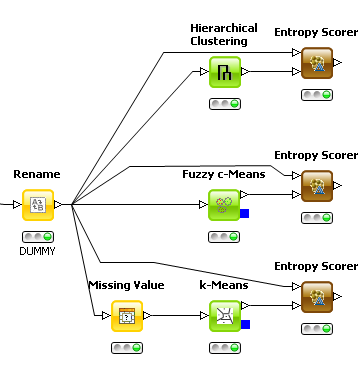
\includegraphics[width=0.5\textwidth]{classification_non_supervisee}
	\caption{Structure des noeuds réalisant la classification non supervisée dans \textsc{knime}}
\end{figure}

Dans un premier temps, on inspecte une mesure de distances en fonction du nombre de clusters hiérarchiques :
\graph{distance_predicted_clusters}{Distance entre clusters en fonction du nombre de clusters demandé (clustering hiérarchique sur les attributs choisis)}
Ce diagramme nous inciterait à chosir 4 clusters plutôt que les 5 choisis plus haut pour l'indice de liberté. Cependant, il ne permet pas de se prononcer sur l'adéquation des données aux classes de liberté.

\begin{figure}[H]
	\centering
	\subfloat[Hiérarchique]{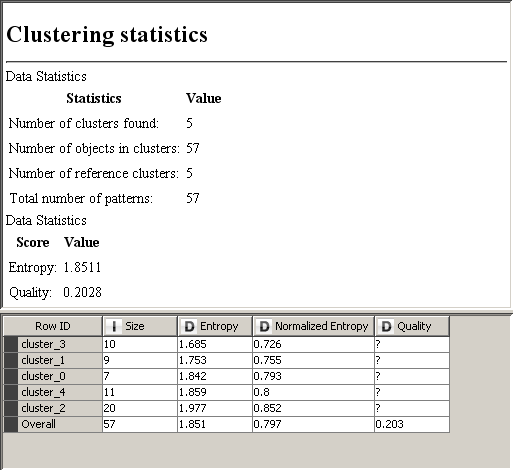
\includegraphics[width=0.3\textwidth]{entropy_hierarchical}}
	\subfloat[Fuzzy C-Means]{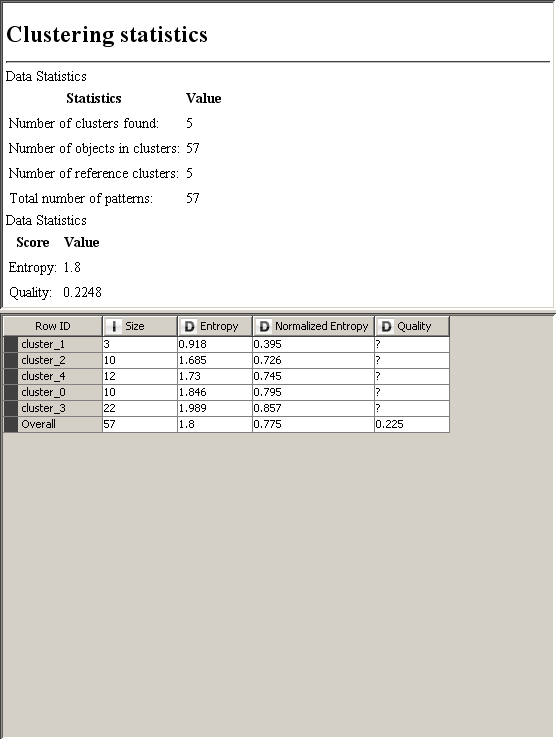
\includegraphics[width=0.3\textwidth]{entropy_fuzzycmeans}}
	\subfloat[K-Means]{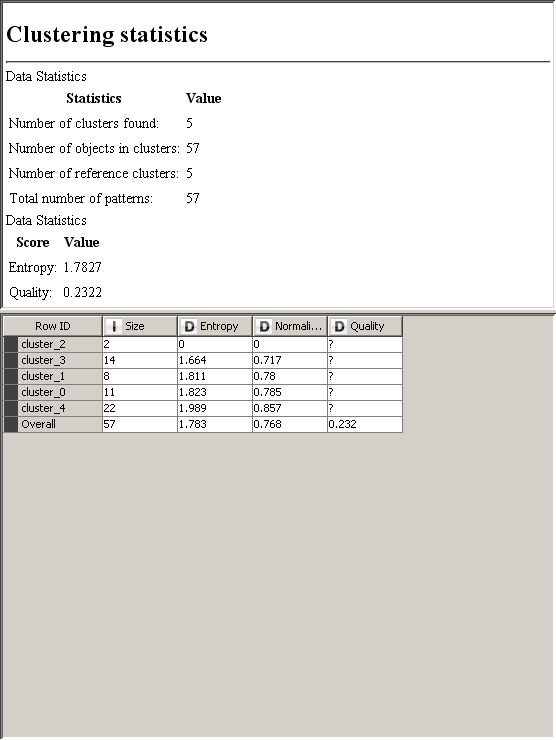
\includegraphics[width=0.3\textwidth]{entropy_kmeans}}
	\caption{Mesure de l'entropie des différents clusterings avec les classes de références}
\end{figure}
C'est un échec. L'entropie est clairement énorme et nous montre que le jeu d'attributs choisi ne constitue pas une base intéressante pour déterminer l'indice de liberté : son clustering n'aboutit à rien de semblable aux classes de liberté.

En étudiant sur les jeux d'attributs \og acceptables à la limite \fg vus plus haut (\emph{Social}, \emph{Armée} et \emph{Economie}), on aboutit au même type de résultats.

%%%%%%%%%%%%%%%%%%%%%%%%%%%%%%%%%%%%%%%%%%%%%%%%%%%%%%%%%%%%
%%%%%%%%%%%%%%%%%%%%%%%%%%%%%%%%%%%%%%%%%%%%%%%%%%%%%%%%%%%%
\section{Classification supervisée}
%%%%%%%%%%%%%%%%%%%%%%%%%%%%%%%%%%%%%%%%%%%%%%%%%%%%%%%%%%%%
%%%%%%%%%%%%%%%%%%%%%%%%%%%%%%%%%%%%%%%%%%%%%%%%%%%%%%%%%%%%
Le principe est cette fois de réaliser un arbre décisionnel qui synthétisera la relation entre classe de liberté et les autres attributs. Compte tenus des résultat obtenus en classification non supervisée, il est probable que cette tentative n'aboutisse pas.

\begin{figure}[H]
	\centering
	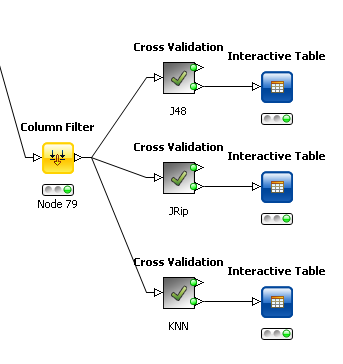
\includegraphics[width=0.5\textwidth]{classification_supervisee}
	\caption{Structure des noeuds réalisant la classification supervisée dans \textsc{knime}}
\end{figure}


On obtient les statistiques d'erreurs suivantes.
\begin{figure}[H]
	\centering
	\subfloat[J48]{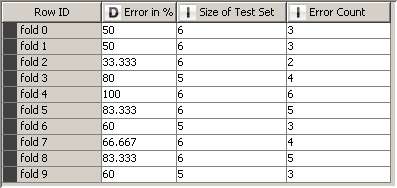
\includegraphics[width=0.3\textwidth]{errors_j48}}
	\subfloat[JRip]{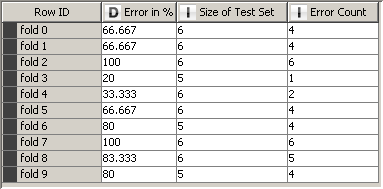
\includegraphics[width=0.3\textwidth]{errors_jrip}}
	\subfloat[KNN]{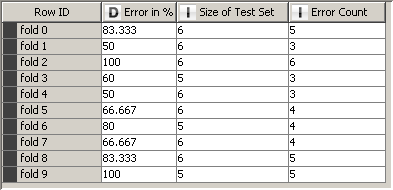
\includegraphics[width=0.3\textwidth]{errors_knn}}
	\caption{Mesure du taux d'erreur des arbres décisionnels obtenus via 3 méthodes}
\end{figure}

Encore une fois, on constate de très mauvais résultats. Les tests aboutissent à de nombreuses erreurs (souvent plus de 50\%), ce qui, pour un ensemble de 5 clusters, est à peine meilleur qu'un choix aléatoire.


%%%%%%%%%%%%%%%%%%%%%%%%%%%%%%%%%%%%%%%%%%%%%%%%%%%%%%%%%%%%
%%%%%%%%%%%%%%%%%%%%%%%%%%%%%%%%%%%%%%%%%%%%%%%%%%%%%%%%%%%%
\section{Conclusion}
%%%%%%%%%%%%%%%%%%%%%%%%%%%%%%%%%%%%%%%%%%%%%%%%%%%%%%%%%%%%
%%%%%%%%%%%%%%%%%%%%%%%%%%%%%%%%%%%%%%%%%%%%%%%%%%%%%%%%%%%%
Nos travaux auront donc permis de déterminer une chose : les liens entre liberté civile d'un peuple et conditions sociale, démographique, économique, etc. sont ténus sur l'ensemble des pays étudiés. On peut donc envisager deux conclusions :
\begin{enumerate}
	\item Soit la liberté de ces peuples n'influence aucunement ces conditions,
	\item soit elle l'influence de plusieurs manières différentes, voire contradictoires, dans plusieurs sous-ensembles de ces pays.
\end{enumerate}
N'ayant pu déterminer des groupes cohérents ni des données concluantes vérifiant la deuxième hypothèse, nous ne pouvons plus nous avancer.

D'un point de vue plus personnel, cette étude nous a appris combien le choix des attributs de départ est important, mais difficile et chronophage. Il nous a semblé que c'est là que réside tout le défi d'une fouille de données propre et fructueuse : nous y avons passé beaucoup de temps, mais paradoxalement c'est là que tous les problèmes de l'étude semblent prendre racine.

